ロジスティック回帰とは与えられたデータに対し, ロジスティック関数を当てはめる問題のことである.
\begin{center}
    \begin{tikzpicture}[>=stealth,scale=1.4]
        \draw[->] (-0.3,0)--(5.5,0) node[right] {$x$};
        \draw[->] (0,-0.3)--(0,4) node[above] {$y$};
        \draw[domain=0:5.5,thick] plot(\x,{3/(1+exp(-3*\x+8))});
        \draw[draw=gray] (5.5,3)--(0,3) node[left] {1};
        \filldraw[fill=white] (0.5,0) circle[radius=0.07];
        \filldraw[fill=white] (1,0) circle[radius=0.07];
        \filldraw[fill=white] (1.5,0) circle[radius=0.07];
        \filldraw[fill=white] (2,0) circle[radius=0.07];
        \filldraw[fill=white] (2.5,3) circle[radius=0.07];
        \filldraw[fill=white] (3,3) circle[radius=0.07];
        \filldraw[fill=white] (3.5,0) circle[radius=0.07];
        \filldraw[fill=white] (4.5,3) circle[radius=0.07];
        \filldraw[fill=white] (5,3) circle[radius=0.07];
        \node at(-0.2,-0.2)  {O};
        \node at(6.3,2) {\large ロジスティック関数};
        \node at(6.3,1.5) {$\displaystyle \tilde{y}_{i}=f(x_{i};a,x_{0})=\frac{1}{1+{\rm exp}(-a(x_{i}-x_{0}))}$};
        \draw[<->,draw=red,thick] (2.5,2.93)--(2.5,1.132);
        \draw[<->,draw=red,thick] (3.5,0.07)--(3.5,2.77);
    \end{tikzpicture}
\end{center}
上のロジスティック関数は関数の値が$y_{i}=\{0,\,1\}$のときに用いられる.\\
以下のように識別機の学習を適用することが出来る.
\begin{eqnarray*}
    クラスA \Leftrightarrow y_{i}=0,\ クラスB \Leftrightarrow y_{i}=1;\\
    {\rm if}(f(x)<0.5)\  {\rm then} クラスA;\  {\rm else} クラスB
\end{eqnarray*}
一般にロジスティック関数は以下で定式化される.
\begin{align*}
    &\frac{dN}{dt}= a\left(\frac{K-N}{K}\right) N \\
    \Longleftrightarrow\ & N(x)=\frac{K}{1+{\rm exp}(-aK(x-x_{0}))}  \tag{3.1}
\end{align*}

\begin{center}
    \begin{tikzpicture}[>=stealth,scale=1.2]
        \draw[domain=-4:4,draw=orange,thick] plot(\x,{3/(1+exp(-2*\x))});
        \draw[domain=-4:4,draw=gray!40] plot(\x,{3/(1+exp(-1*\x))});
        \draw[domain=-4:4,draw=gray!80] plot(\x,{3/(1+exp(-1.7*\x))});
        \draw[domain=-4:4,draw=gray!60] plot(\x,{3/(1+exp(-2.2*\x))});
        \draw[domain=-3:2.5,draw=blue!60,thick] plot(\x+1.5,{3/(1+exp(-2*(\x)))});
        \draw[domain=-4:4,draw=red,dashed,thick] plot(\x,{2.3/(1+exp(-2*\x))});
        \draw[draw=gray!80] (4,3)--(0,3) node[left]{$K$};
        \draw(0,1.5)--(0,1.5) node[left] {$K/2$};
        \draw[draw=gray!80,dashed] (4,2.3)--(0,2.3)  node[left] {1};
        \draw[->,draw=magenta](0,1.5)--(1.5,1.5);
        \draw[->](-4,0)--(4,0) node[right]{$x$};
        \draw[->](0,-0.3)--(0,4) node[above]{$y$};
        \node at(-0.2,-0.2) {O};
        \node at(4,2) {\textcolor{red}{シグモイド関数}};
        \node at(4,3.3) {\textcolor{blue}{ロジスティック関数}};
    \end{tikzpicture}
\end{center}
シグモイド関数は, ロジスティック関数の$K=1,\,x_{0}=0$の特殊な場合に相当する.\\
(標準)シグモイド関数は以下の式で表すことができる.
\begin{align*}
    f(x)=\frac{1}{1+{\rm exp}(-x)} \tag{3.2}
\end{align*}
シグモイド関数において, $a$の値によって, 関数の傾き度合いが変わる.
\begin{center}
    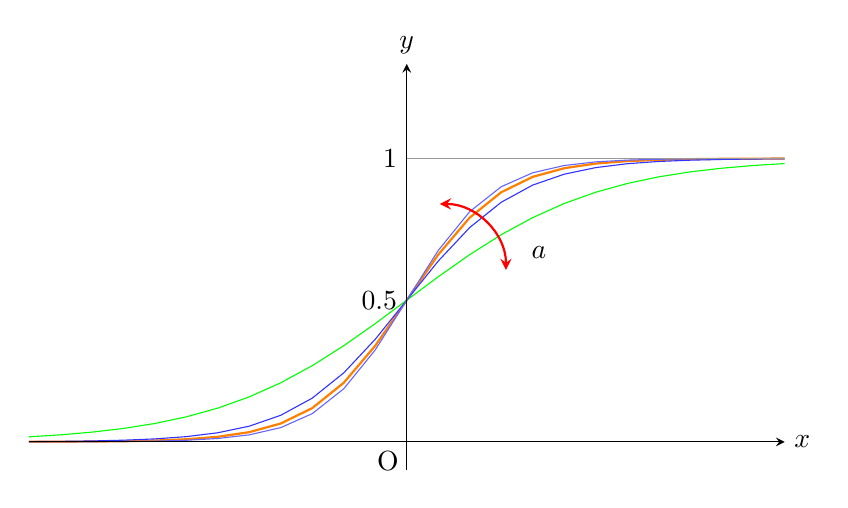
\begin{tikzpicture}[>=stealth,scale=1.2]
        \draw[domain=-4:4,draw=orange,thick] plot(\x,{3/(1+exp(-2*\x))});
        \draw[domain=-4:4,draw=green] plot(\x,{3/(1+exp(-1*\x))});
        \draw[domain=-4:4,draw=blue!80] plot(\x,{3/(1+exp(-1.7*\x))});
        \draw[domain=-4:4,draw=blue!60] plot(\x,{3/(1+exp(-2.2*\x))});
        \draw[draw=gray!80] (4,3)--(0,3) node[left]{$1$};
        \draw(0,1.5)--(0,1.5) node[left] {$0.5$};
        \draw[->](-4,0)--(4,0) node[right]{$x$};
        \draw[->](0,-0.3)--(0,4) node[above]{$y$};
        \node at(-0.2,-0.2) {O};
        \draw[<->,draw=red,thick](60:2.1) arc(0:90:0.7cm);
        \node at(1.4,2) {$a$};
    \end{tikzpicture}
\end{center}
シグモイド関数を$x$軸に$b$だけシフトしたときの関数は以下のように表すことが出来る.
\begin{align*}
    f(x) = \frac{1}{1+{\rm exp}(-a(x-b))}
\end{align*}
すると以下のようにグラフは描くことが可能となる.
\begin{center}
    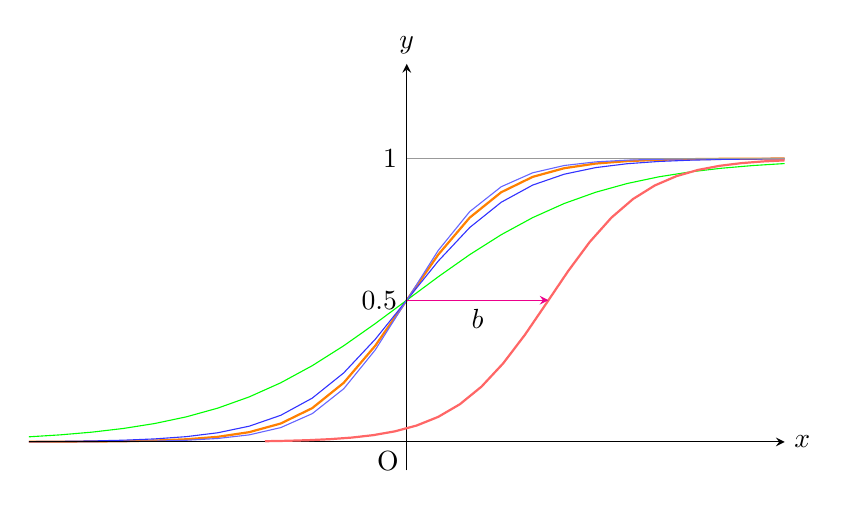
\begin{tikzpicture}[>=stealth,scale=1.2]
        \draw[domain=-4:4,draw=orange,thick] plot(\x,{3/(1+exp(-2*\x))});
        \draw[domain=-4:4,draw=green] plot(\x,{3/(1+exp(-1*\x))});
        \draw[domain=-4:4,draw=blue!80] plot(\x,{3/(1+exp(-1.7*\x))});
        \draw[domain=-4:4,draw=blue!60] plot(\x,{3/(1+exp(-2.2*\x))});
        \draw[draw=gray!80] (4,3)--(0,3) node[left]{$1$};
        \draw(0,1.5)--(0,1.5) node[left] {$0.5$};
        \draw[->](-4,0)--(4,0) node[right]{$x$};
        \draw[->](0,-0.3)--(0,4) node[above]{$y$};
        \node at(-0.2,-0.2) {O};
        \draw[domain=-3:2.5,draw=red!60,thick] plot(\x+1.5,{3/(1+exp(-2*(\x)))});
        \draw[->,draw=magenta](0,1.5)--(1.5,1.5);
        \node at(0.75,1.3) {$b$};
    \end{tikzpicture}
\end{center}
シグモイド関数の重要な性質として微分が元の関数を用いて表現することができる.
\begin{eqnarray*}
    f'(x)&=&\left(\frac{1}{1+{\rm exp}(-x)}\right)'\\
        &=&\frac{{\rm exp}(-x)}{\left(1+{\rm exp}(-x)\right)^{2}}\\
        &=&\frac{1}{1+{\rm exp}(-x)}\cdot \frac{{\rm exp}(-x)}{1+{\rm exp}(-x)}\\
        &=&\frac{1}{1+{\rm exp}(-x)}\cdot \frac{1+{\rm exp}(-x)-1}{1+{\rm exp}(-x)}\\
        &=&\frac{1}{1+{\rm exp}(-x)}\cdot \left(1-\frac{1}{1+{\rm exp}(-x)}\right)\\
        &=&f(x)\left(1-f(x)\right)
\end{eqnarray*}
また, $f'''(x)$については
\begin{eqnarray*}
    f''(x) &=& \left(f'(x)\right)'\\
        &=& \left(f(x)(1-f(x))\right)'\\
        &=& f'(x)(1-f(x))+f(x)(1-f(x))'\\
        &=& f'(x)(1-f(x))-f(x)f'(x)\\
        &=& f'(x)(1-2f(x))\\
        &=& f(x)(1-f(x))(1-2f(x))
\end{eqnarray*}
よって,まとめると
\begin{align*}
    f(x) &= \frac{1}{1+{\rm exp}(-x)}\\
    f'(x)&=f(x)(1-f(x)) \tag {3.3} \\
    f''(x)&=f(x)(1-f(x))(1-2f(x))
\end{align*}
$(x_{n},y_{n})$\ :\ $n$番目の学習データ\\
$\mbox{\boldmath $x$}_{n}=\begin{bmatrix} x_{n}&1 \end{bmatrix}^{T}$\ :\ $x_{n}$を次元拡張してベクトル化したもの\\
$D=\begin{bmatrix}\mbox{\boldmath $x$}_{1}&\mbox{\boldmath $x$}_{2}&\cdots &\mbox{\boldmath $x$}_{n}&\cdots \end{bmatrix}^{T}=\begin{bmatrix}d_{ij}\end{bmatrix},\ (d_{i1}=x_{i},\,d_{i2}=1)$\\
$z_{n}=\mbox{\boldmath $w$}^{T}\mbox{\boldmath $x$}_{n}=\displaystyle \sum_{k}w_{k}\cdot d_{nk}$\\
ここで線形回帰の場合は$\tilde{y}_{n}=f(x_{i};a,b)=ax_{i}+b$としていたが, ロジスティック回帰では\\
$\tilde{y}_{n}=f(z_{n})=\displaystyle \frac{1}{1+{\rm exp}(-z_{n})}$\\[0.1cm]
$\displaystyle E=\frac{1}{2}\sum_{n=1}^{N}(y_{n}-\tilde{y}_{n})^{2}=\frac{1}{2}\sum_{n=1}^{N}\left(y_{n}-\frac{1}{1+{\rm exp}(-z_{n})}\right)^{2}$\\[1cm]
これから誤差$E$が最小となるように計算していくが, ロジスティック回帰の場合は解が解析的に求まらない(微分方程式の解が定まらない)ので, \textcolor{red}{繰り返し計算}が必要となる.\\
ここで, {\bf 勾配法}というものを導入する.